% either Uni Rostock style
\documentclass[mathserif, aspectratio=43]{intbeamer}
\setbeamertemplate{page number in head/foot}[parts]
\AtBeginPart{\makepart\setcounter{framenumber}{0}}
\addtobeamertemplate{block begin}{
\setlength{\textwidth}{0.98\textwidth}}{}

% or some beamer theme
% \documentclass[aspectratio=43]{beamer}
% \usetheme{Boadilla}
% \usecolortheme{dove}
% \setbeamertemplate{navigation symbols}{}
% \usefonttheme[onlymath]{serif}
% \addtobeamertemplate{headline}{}{\insertsection}


% required packages
\usepackage[utf8]{inputenc}
\usepackage[english]{babel}
\usepackage{graphicx}
\usepackage{xcolor}
\usepackage{amsmath}
\usepackage{amsfonts}
\usepackage{amssymb}
\usepackage{amsbsy}
\usepackage{bm}
\usepackage{trfsigns}
\usepackage{tikz}
\usepackage{comment}

\newcommand\fsd{\mathrm{d}} %der/int operator

% shorten figure caption
\addto\captionsenglish{\renewcommand{\figurename}{Fig.}}
%\addto\captionsngerman{\renewcommand{\figurename}{Abb.}}

%matplotlib colors:
\definecolor{C0}{HTML}{1f77b4}
\definecolor{C1}{HTML}{ff7f0e}
\definecolor{C2}{HTML}{2ca02c}
\definecolor{C3}{HTML}{d62728}
\definecolor{C7}{HTML}{7f7f7f}

\title[UE SigSys]{Übung \\ \huge Signal- und Systemtheorie}
\author[Schultz, INT, IEF, Uni Rostock]{Frank Schultz}
\date[SS 2021]{Sommersemester 2021}

\begin{document}
\maketitle
\section{UE 00}
% TBD

%\begin{comment}



\section{UE 01 / 2021-04-14}
%
\begin{frame}{UE 01 Schedule / Objectives}
Signals
\begin{itemize}
\item The Four Fourier Transforms (FTs)
\item Basics Fourier Series (Sinc / Rect duality)
\item Basics Fourier Transform (Sinc / Rect duality)
\item Fundamental FT Correspondences
\end{itemize}
Systems
\begin{itemize}
\item The Dirac Impulse
%\item From Dirac Impulse to the Green's Function of ODEs =
\item From Dirac Impulse to the Impulse Response of an LTI System
\end{itemize}
\end{frame}




\begin{frame}{Fourier Reihe / Fourier Series (FS)}
\begin{itemize}
\item for continuous-time, periodic signals $x(t)\in\mathbb{C}$
with signal period $T_0$, fundamental (physical) frequency $f_0=\frac{1}{T_0}$
\item in SigSys we rather use angular frequency, i.e. $\omega_0 = 2 \pi f_0 = \frac{2\pi}{T_0}$
\item analysis (i.e. get Fourier coefficients $\tilde{X}$ over $\mu\in\mathbb{Z}$)
$$\tilde{X}[\mu] =
\int\limits_{0}^{T_0} x(t) \, \e^{-\im \frac{2\pi}{T_0} \mu t}\,\mathrm{d}t =
\int\limits_{0}^{T_0} x(t) \, \e^{-\im \omega_0 \mu t}\,\mathrm{d}t$$
\item synthesis (i.e. linear combination)
$$x(t) =
\frac{1}{T_0}\sum\limits_{\mu=-\infty}^{+\infty} \tilde{X}[\mu] \,\e^{+\im \frac{2\pi}{T_0} \mu t} =
\frac{1}{T_0}\sum\limits_{\mu=-\infty}^{+\infty} \tilde{X}[\mu] \,\e^{+\im \omega_0 \mu t}
$$
\item note: $T$ and $c_k T$ in tutorial corresponds to $T_0$ and $\tilde{X}[\mu]$ here in slides
\end{itemize}
\end{frame}




\begin{frame}{Fourier Transform (FT)}
\begin{itemize}
\item for continuous-time signals $x(t)\in\mathbb{C}$
\item analysis (i.e. FT spectrum over $\omega\in\mathbb{R}$)
$$X(\im\omega) = \int\limits_{-\infty}^{+\infty} x(t) \,\e^{-\im \omega t}\,\mathrm{d}t$$
\item synthesis
$$x(t) = \frac{1}{2\pi}\int\limits_{-\infty}^{+\infty} X(\im\omega) \,\e^{+\im \omega t}\,\mathrm{d}\omega
$$
\item FT operator symbol $$x(t) \,\laplace\,  X(\im\omega)$$
\end{itemize}
\end{frame}



\begin{frame}{Discrete-Time Fourier Transform (DTFT)}
\begin{itemize}
\item for discrete-time signals $x[k]\in\mathbb{C}$, $k\in\mathbb{Z}$
\item analysis (i.e. DTFT spectrum over $\Omega\in\mathbb{R}$)
$$X(\e^{\im\Omega}) = \sum\limits_{k=-\infty}^{+\infty} x[k] \,\e^{-\im \Omega k}$$
\item synthesis
$$x[k] = \frac{1}{2\pi}\int\limits_{0}^{2\pi} X(\e^{\im\Omega}) \,\e^{+\im \Omega k}\,\mathrm{d}\Omega
$$
\end{itemize}
\end{frame}






\begin{frame}{Discrete Fourier Transform (DFT)}
%
\begin{itemize}
\item for discrete-time, periodic signals $x[k]\in\mathbb{C}$, $k\in\mathbb{Z}$
with signal period $N$ samples
\item analysis (i.e. DFT coefficients over $\mu\in\mathbb{Z}$)
$$X[\mu] = \sum\limits_{k=0}^{N-1} x[k] \,\e^{-\im \frac{2\pi}{N} \mu k} =
\sum\limits_{k=0}^{N-1} x[k] \,\e^{-\im \Omega_0 \mu k}$$
\item synthesis
$$x[k] = \frac{1}{N}\sum\limits_{\mu=0}^{N-1} X[\mu] \,\e^{+\im \frac{2\pi}{N} \mu k} =
\frac{1}{N}\sum\limits_{\mu=0}^{N-1} X[\mu] \,\e^{+\im \Omega_0 \mu k}$$
\item with fundamental DFT frequency $\Omega_0 = \frac{2\pi}{N}$
\end{itemize}
%
\end{frame}








\begin{frame}{Fourier Series for Periodic Rect Impulse}
Task 1.1
\begin{figure}
\includegraphics[width=\textwidth]{../fs/D1483A84E2_0.pdf}
\caption{1.1}
\end{figure}
\end{frame}

\begin{frame}{Fourier Series for Periodic Rect Impulse}
Task 1.1
\begin{figure}
\includegraphics[width=\textwidth]{../fs/D1483A84E2_1.pdf}
\caption{1.2}
\end{figure}
\end{frame}

\begin{frame}{Fourier Series for Periodic Rect Impulse}
Task 1.1
\begin{figure}
\includegraphics[width=\textwidth]{../fs/D1483A84E2_2.pdf}
\caption{1.3}
\end{figure}
\end{frame}

\begin{frame}{Fourier Series for Periodic Rect Impulse}
Task 1.1
\begin{figure}
\includegraphics[width=\textwidth]{../fs/D1483A84E2_3.pdf}
\caption{1.4}
\end{figure}
\end{frame}

\begin{frame}{Fourier Series for Periodic Rect Impulse}
Task 1.1
\begin{figure}
\includegraphics[width=\textwidth]{../fs/D1483A84E2_4.pdf}
\caption{1.5}
\end{figure}
\end{frame}


\begin{frame}{Fourier Transform for Single Rect Impulse}
Task 1.2
\begin{figure}
\includegraphics[width=0.7\textwidth]{../ft/8C3958BE4F_1.pdf}
\includegraphics[width=0.7\textwidth]{../ft/8C3958BE4F_0.pdf}
\caption{1.6}
\end{figure}
\end{frame}



\begin{frame}{Fourier Transform Spectrum -> Magnitude / Phase Plot}
Task 1.2
\begin{figure}
\includegraphics[width=0.7\textwidth]{../ft/8C3958BE4F_SingleCase_MagPhase.pdf}
\caption{1.7}
\end{figure}
\end{frame}


\begin{frame}{Fourier Transform Rect / Sinc Duality}
For our used definition of the rect function (Rechteckimpuls)
$$\text{rect}(t) := \begin{cases} 1 & |t| < \frac{1}{2} \\ \frac{1}{2} & |t| = \frac{1}{2} \\ 0 & |t| > \frac{1}{2} \end{cases}$$
and of the sinc function (Spaltfunktion)
$$\text{sinc}(t) := \frac{\sin(t)}{t}$$
the duality
$$\text{rect}(t) \,\laplace\,  \,\,\,\text{sinc}\left( \frac{\omega}{2} \right)$$
$$\text{sinc}(t) \,\laplace\, \pi \,\text{rect}\left(\frac{\omega}{2}\right)$$
is of fundamental importance in SigSys
\end{frame}



\begin{frame}{Fourier Transform for Right-Shifted Single Rect Impulse}
Task 1.3: Time Shift Leads to Phase Change
\begin{figure}
\includegraphics[width=0.7\textwidth]{../ft/A8A2DEE53A.pdf}
\caption{1.8}
\end{figure}
\end{frame}



\begin{frame}{Fourier Transform for Left-Shifted Single Rect Impulse}
Task 1.4: here special also time-reversed signal of Task 1.3
\begin{figure}
\includegraphics[width=0.7\textwidth]{../ft/1CFE5FE3A1.pdf}
\caption{1.9}
\end{figure}
\end{frame}



\begin{frame}{Fourier Transform Time / Phase Reversal}
%
from Task 1.3 and 1.4 we find
\begin{align*}
x(+t) \quad \laplace \quad X(+\im\omega) =& |X(\im\omega)| \, \e^{+\im\angle X(\im\omega)}\\
x(-t) \quad \laplace \quad X(-\im\omega) =& |X(\im\omega)| \, \e^{-\im\angle X(\im\omega)}
\end{align*}
%
\begin{figure}
\includegraphics[width=0.49\textwidth]{../ft/A8A2DEE53A.pdf}
\includegraphics[width=0.49\textwidth]{../ft/1CFE5FE3A1.pdf}
\caption{1.8 \& 1.9}
\end{figure}
%
\end{frame}




\begin{frame}{Fourier Transform Shift / Modulation Duality}
%
\textbf{Zeitverschiebung} um $\tau\in\mathbb{R}$ aka \textbf{Verschiebungssatz}
\begin{align*}
x(t) & \quad \laplace \quad X(\im\omega)\\
x(t - \tau) & \quad \laplace \quad X(\im\omega) \cdot \e^{-\im\omega \tau}
\end{align*}
%
\textbf{Frequenzverschiebung} um $\omega_0\in\mathbb{R}$ aka \textbf{Modulationssatz}
(see Task 1.5)
\begin{align*}
x(t) & \quad \laplace \quad X(\im\omega)\\
\label{eq:A8A2DEE53A_ModTheoremTime}
x(t) \cdot \e^{+\im\omega_0 t} & \quad \laplace \quad X(\im[\omega-\omega_0])
\end{align*}
%
Wie sind die Fourier Transformationen von
\begin{align*}
\cos(\omega_0 t) = \frac{\e^{+\im\omega_0 t}+\e^{-\im\omega_0 t}}{2}\qquad
\sin(\omega_0 t) = \frac{\e^{+\im\omega_0 t}-\e^{-\im\omega_0 t}}{2\im}\quad??
\end{align*}
\end{frame}















\begin{frame}{Dirac Impulse And Sifting Property}
Task 1.6:
%
%\begin{equation*}
%\label{eq:DiracDistrDef}
$\lim_{\xi\to\infty} \int\limits_{-\infty}^{+\infty}
\delta_\xi(t-t_0) \cdot f(t) \, \fsd t
:= \int\limits_{-\infty}^{+\infty} \delta(t-t_0) \cdot f(t) \, \fsd t \stackrel{\mathrm{def}}= f(t_0)$
%\end{equation*}
%
\begin{figure}
\includegraphics[width=0.6\textwidth]{../dirac_impulse_ct/D410BDAAE0.pdf}
\caption{1.10, top: Rect, bottom: normalized Sinc}
\end{figure}
\end{frame}




\begin{frame}{Dirac Impulse And Sifting Property}
Task 1.6

\begin{itemize}
\item we define Dirac Delta impulse by $\delta(t)$ for the following equation
%
\item
$\lim_{\xi\to\infty} \int\limits_{-\infty}^{+\infty}
\delta_\xi(t-t_0) \cdot f(t) \, \fsd t
:= \int\limits_{-\infty}^{+\infty} \delta(t-t_0) \cdot f(t) \, \fsd t \stackrel{\mathrm{def}}= f(t_0)$
%
\item again: right integral equation is not a Riemann integral, but a definition
%
\item from that definition we directly find special cases
%
$$\int\limits_{-\infty}^{+\infty} \delta(t) \cdot f(t) \, \fsd t = f(0) \qquad\text{for}\qquad t_0=0$$
%
$$\int\limits_{-\infty}^{+\infty} \delta(t) \fsd t = 1
\qquad\text{for}\qquad f(t)=1$$
%
\end{itemize}
%
\end{frame}


















\begin{frame}{Fourier Transform Duality for Dirac Impulse}

\begin{figure}[h!]
\centering
%
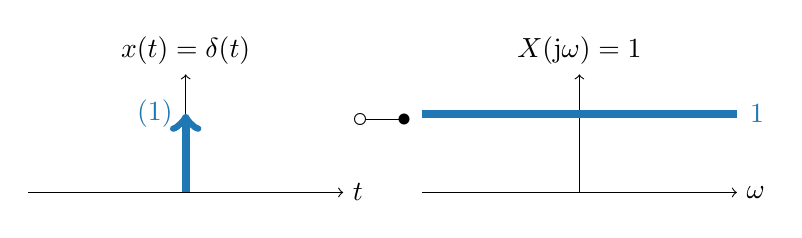
\begin{tikzpicture}0
\def\l{-2.5}
\def\r{+2.5}
\draw[->] (-2+\l,0) -- (2+\l,0) node[right] {$t$};
\draw[->] (0+\l,0) -- (0+\l,1.5) node[above] {$x(t)=\delta(t)$};
\draw[->, C0, line width=1mm] (0+\l,0) -- (0+\l,1) node[left] {$(1)$};
\node at (0,1) {$\laplace$};
\draw[->] (-2+\r,0) -- (2+\r,0) node[right] {$\omega$};
\draw[->] (0+\r,0) -- (0+\r,1.5) node[above] {$X(\im\omega)=1$};
\draw[-, C0, line width=1mm] (-2+\r,1) -- (2+\r,1) node[right] {$1$};
\end{tikzpicture}
%
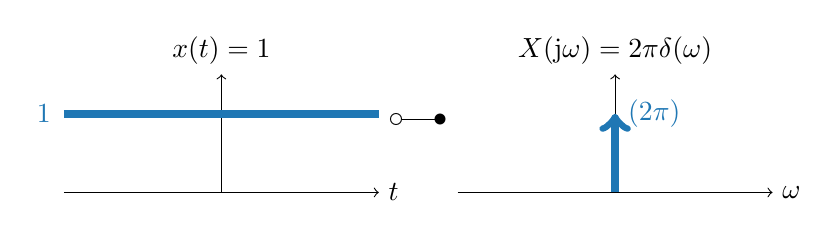
\begin{tikzpicture}0
\def\l{-2.5}
\def\r{+2.5}
\draw[->] (-2+\l,0) -- (2+\l,0) node[right] {$t$};
\draw[->] (0+\l,0) -- (0+\l,1.5) node[above] {$x(t)=1$};
\draw[-, C0, line width=1mm] (-2+\l,1) node[left] {$1$} -- (2+\l,1);
\node at (0,1) {$\laplace$};
\draw[->] (-2+\r,0) -- (2+\r,0) node[right] {$\omega$};
\draw[->] (0+\r,0) -- (0+\r,1.5) node[above] {$X(\im\omega)=2\pi\delta(\omega)$};
\draw[->, C0, line width=1mm] (0+\r,0) -- (0+\r,1) node[right] {$(2\pi)$};
\end{tikzpicture}
%
\caption{1.11}
\end{figure}

\end{frame}



\begin{frame}{Most Important Fourier Transform Properties}
%
as of now we know so far
\begin{align*}
x(t)= \delta(t) &\quad \laplace \quad X(\im\omega)=1\\
x(t)= 1 &\quad \laplace \quad X(\im\omega)=2\pi \delta(\omega)\\
x(t - \tau) & \quad \laplace \quad X(\im\omega) \cdot \e^{-\im\omega \tau}\\
x(t) \cdot \e^{+\im\omega_0 t} & \quad \laplace \quad X(\im[\omega-\omega_0])
\end{align*}
%
from these we can deduce further nice properties
\begin{align*}
\delta(t-\tau)& \quad \laplace \quad 1 \cdot \e^{-\im\omega \tau}\\
1 \cdot \e^{+\im\omega_0 t} & \quad \laplace \quad 2\pi\delta(\omega-\omega_0)
\end{align*}
%
Jetzt können wir 'lösen': Wie sind die Fourier Transformationen von
\begin{align*}
\cos(\omega_0 t) = \frac{\e^{+\im\omega_0 t}+\e^{-\im\omega_0 t}}{2}\qquad
\sin(\omega_0 t) = \frac{\e^{+\im\omega_0 t}-\e^{-\im\omega_0 t}}{2\im}\quad??
\end{align*}
%
\end{frame}



\begin{frame}{Impulse Response of System, Green's Function of ODE}
Task 1.7: Find the solution $y(t)$ for $t\geq 0$ of the ODE and given initial conditions
$$\frac{16}{25} \ddot{y}(t) + \frac{24}{25} \dot{y}(t) + y(t) = 0,
\quad y(0)=0,\quad \dot{y}(0)=\frac{25}{16}$$
The solution is known as impulse response $h(t)$ in SigSys
$$h(t) := y(t) = \frac{25}{16} \e^{-\frac{3}{4} t} \sin(t), \qquad t\geq 0$$
since the problem is equivalent with excitation $x(t) = \delta(t)$
$$A \ddot{y}(t) + B \dot{y}(t) + C y(t) = \delta(t),\qquad {y}(0_-) = 0,\qquad \dot{y}(0_-) = 0$$
%
Convolution integral using impulse response for any other $x(t \leq 0)$
$$y_p(t) = \int\limits_{0}^{t} h(t-\tau) x(\tau) \fsd \tau$$
%
\end{frame}

%\end{comment}





\section{UE 02 / 2021-04-21}
\begin{frame}{UE 02 Schedule / Objectives}

\begin{itemize}
\item Elementarsignale
\item Signaloperationen im Detail
\item Testen von Systemen auf Linearität und Zeitinavarianz (LTI)
\item Why and How To Faltung? ET Beispiele
\end{itemize}

\end{frame}
% \section{UE 03}
% \begin{frame}{}
% %
% \end{frame}
% \section{UE 04}
% \begin{frame}{}
% %
% \end{frame}
% \section{UE 05}
% \begin{frame}{}
% %
% \end{frame}
% \section{UE 06}
% \begin{frame}{}
% %
% \end{frame}
% \section{UE 07}
% \begin{frame}{}
% %
% \end{frame}
% \section{UE 08}
% \begin{frame}{}
% %
% \end{frame}
% \section{UE 09}
% \begin{frame}{}
% %
% \end{frame}
% \section{UE 10}
% \begin{frame}{}
% %
% \end{frame}
% \section{UE 11}
% \begin{frame}{}
% %
% \end{frame}
% \section{UE 12}
% \begin{frame}{}
% %
% \end{frame}
% \section{UE 13}
% \begin{frame}{}
% %
% \end{frame}
%
\end{document}
